\chapter*{Descrizione Progetto}
\renewcommand{\thesection}{\arabic{section}}
Lo scopo di questo progetto consiste nella valutazione dei costi operativi di un call center con operatività 24 ore su 24, 7 giorni su 7 per conto di un'azienda del settore utilities.
Nel nostro caso è stato scelto di analizzare le stime degli \ac{OPEX} riguardanti i primi mesi a partire dell'apertura del call center nell'anno solare 2016.
\section[Sede legale e fiscale]{Sede legale e fiscale}
La locazione della sede legale e fiscale è stata scelta in Albania, più precisamente nella capitale Tirana.
La scelta di questo paese extracomunitario, anche se in procinto di entrare nella \ac{UE}\cite{entrataAlbaniaUE}, risiede principalmente:
\begin{itemize}
	\item in un \textbf{sistema fiscale} che favorisce l'investimento di capitali esteri;
	\item un \textbf{cambio favorevole}. La moneta locale, il \textit{lek} (\textbf{ALL}), presenta il seguente tasso di cambio (dati aggiornati al 15/12/2016):
	\begin{center}
		1 \euro : 136,51 ALL
	\end{center}
	Per nostra semplicità abbiamo eseguito i nostri calcoli in \textit{euro} tenendo conto del tenore di vita a Tirana.
	\item nella sua \textbf{posizione geografica strategica}. L'Albania è uno stato della penisola balcanica, confinante con il Montenegro a nord-ovest, il Kosovo a nord-est, la Macedonia ad est e a sud con la Grecia. Si affaccia sul Mar Adriatico (sul Canale d'Otranto) e sul Mar Ionio che lo separa dall'Italia (circa 60km).
\end{itemize} 
\section[Sistema Fiscale]{Sistema Fiscale}
  
\subsection[Persone Giuridiche]{Persone Giuridiche}
Una persona giuridica, ovvero un ente il cui ordinamento giuridico attribuisce la \textit{capacità giuridica} (diventando, quindi, un \textbf{soggetto di diritto}) è considerata come residente in Albania se ha una struttura permanente, la sede principale, o una sede per la reale gestione degli affari nel Paese.
\subsubsection{Imposta sul reddito aziendale} 
Tutte le imprese che siano albanesi o straniere registrate ai fini \ac{IVA} sono soggette all'\textit{imposta sul reddito aziendale} calcolata sulla base delle seguenti aliquote:
\begin{itemize}
	\item \textbf{15\%}, per le grandi imprese;
	\item \textbf{imposta semplificata} per le piccole imprese o piccoli imprenditori che realizzano un fatturato annuo lordo inferiore di \textbf{ALL 8 milioni} (circa 58603,77\euro). Le aliquote previste sono:
		\begin{center}
 			\begin{tabular}{SS[table-comparator = true]}
 			\toprule 
 				{Aliquota Applicata (\%)} & {Fatturato Annuale(ALL)} \\
 			\midrule
 				5 & \numrange{5000000}{8000000} \\
 				0 & < 5000000 \\
 			\bottomrule
 			\end{tabular} 
		\end{center}
\end{itemize} 
\subsubsection{IVA}
E' applicata sulla vendita delle merci e dei servizi a un tasso standard del 20\% e 10\% sulle medicine. La VAT non si applica sulle
esportazioni e sui servizi internazionali come per esempio il trasporto di merci e passeggeri.
\subsection[Persone Fisiche]{Persone Fisiche}
Una persona fisica, invece, è soggetta al pagamento delle tasse relative ai guadagni realizzati all'interno del territorio albanese, se non è residente, altrimenti deve pagare le tasse su tutti i guadagni realizzati anche all'estero.
Sono previste le seguenti aliquote:\newline
\begin{center}
 \begin{tabular}{SS[table-comparator = true]}
 \toprule
 	{Aliquota Applicata (\%)} & {Reddito Mensile(ALL)} \\
 \midrule
 	0 & < 30000 \\
 	13 & \numrange{30001}{130000} \\
 	23 & > 130001 \\
 \bottomrule
 \end{tabular} 
\end{center}
\section[Gruppo Sistelia]{Gruppo Sistelia}

\subsection[ReteTurismo]{ReteTurismo}

 	\[ y = a * x + b\]

 \begin{tabular}{SS[table-format=2]}
 \toprule
 	{Anno} & {Numero Abbonati} \\
 \midrule
 	2010 & 4515000 \\
 	2011 & 4831000 \\
 	2012 & 4900000 \\
 	2013 & 4700000 \\
 	2014 & 4723000 \\
 	2015 & 4740000 \\
 \bottomrule
 \end{tabular} 

 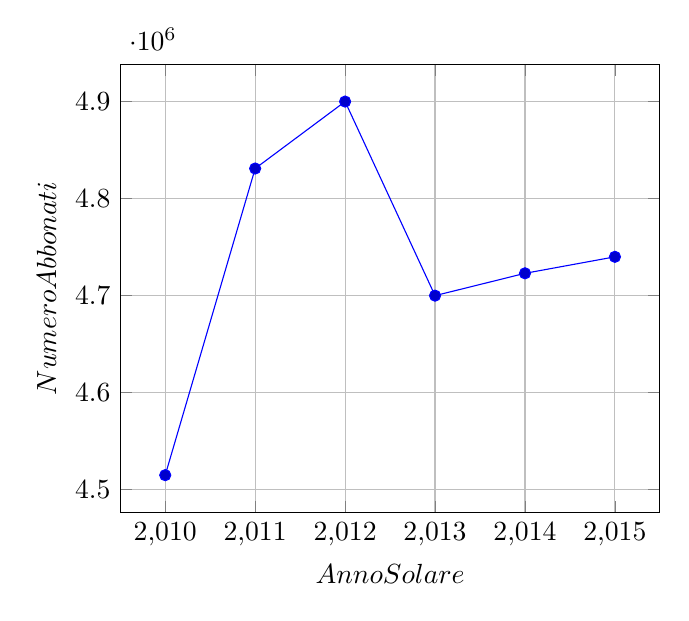
\begin{tikzpicture}
	\begin{axis}[ xlabel=$Anno Solare$, ylabel=$Numero Abbonati$, grid=major	
	]
		
		\addplot coordinates{( 2010, 4515000) 
							  ( 2011, 4831000)
							  ( 2012, 4900000)
							  ( 2013, 4700000)
							  ( 2014, 4723000)
							  ( 2015, 4740000)};
	\end{axis}
\end{tikzpicture}